\section{Method}\label{sec:method}

\subsection{From the elevation model to crest paths}\label{sec:crestpaths}\label{sec:trees}

Figure~\ref{fig:pipeline} shows the steps on the Alps, Table~\ref{tab:counts} what they give, and Appendix~\ref{app:construction}
the detail of each step. Every constant is a named constant of the code, listed in Appendix~\ref{app:params}.

\begin{figure}
\centering
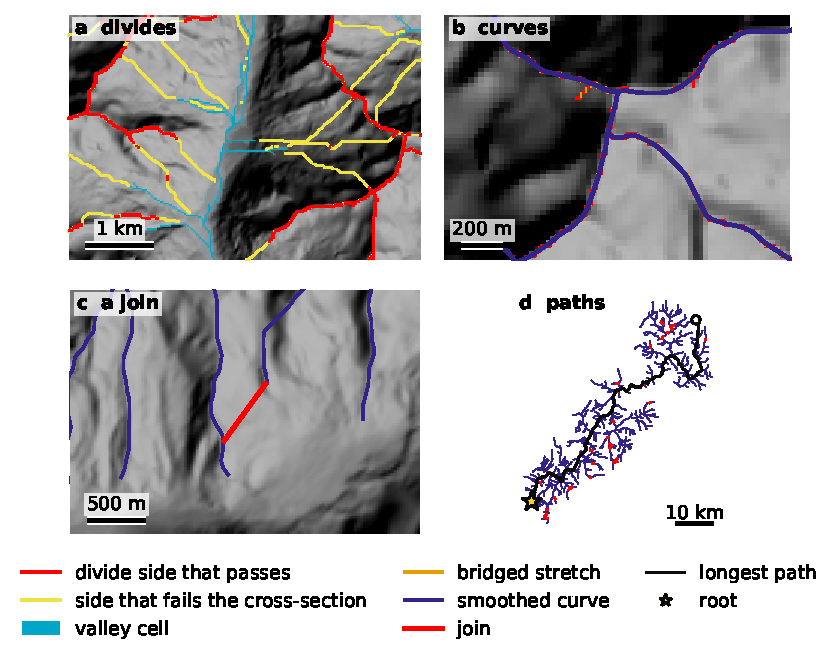
\includegraphics[width=\textwidth]{figures/pipeline.pdf}
\caption{The crests come out of the elevation model in four steps. \textbf{a}~Divide sides on a hillshade of a part of the Écrins:
the sides that pass the two tests are red and those that fail only the cross-section yellow. \textbf{b}~The sides become smooth curves,
bridging flat stretches. \textbf{c}~A join links two curves and stays on the ridge. \textbf{d}~The longest tree of the Alps with its
longest path, from the root (star) to the tip (circle).}
\label{fig:pipeline}
\end{figure}

\paragraph{Ground and mountain area.} The elevations are the IGN BD~ALTI v2 model at 25~m, in Lambert-93. A massif is the set of
the departments of Appendix~\ref{app:params}. Its mountain area follows the UNEP-WCMC classes (Kapos et al.\ 2000~\cite{kapos}) on 1~km cells;
a curve belongs to the massif if at least \CgPMaskShare\% of it lies in this area (Appendix~\ref{app:construction}).

\paragraph{Divides.} After depression filling (Barnes, Lehman and Mulla 2014~\cite{barnes}) and steepest-descent routing, the valleys are the cells that drain at least
\CgPValley~km$^2$. A side between two cells that drain into different valleys, neither downstream of the other, is a divide side. It is a
crest if the ground falls away on both sides. Let $d$ be the unit step from cell $a$ to cell $b$, $z$ the elevation and
$n=\CgPXsecCells$ cells ($\CgPXsecM$~m):
\begin{equation}
  z(a)-z(a-n\,d)\ \ge\ \Delta_z,\qquad z(b)-z(b+n\,d)\ \ge\ \Delta_z,\qquad \Delta_z=\CgPXsecDrop~\mathrm{m}.
  \label{eq:xsec}
\end{equation}
The crest must also stand at least $h_{\min}=\CgPHandMin$~m above the streams.

\paragraph{Curves.} Flat stretches of at most \CgPBridgeSides{} sides that fail only the cross-section are bridged and short dead ends are
pruned. At a junction a curve goes on along the straightest continuation, as a pilot who keeps following the ridge would. A smoothing spline with a
cut-off of \CgPSmooth~m removes the steps of the grid, and the curve is resampled every $\Delta s=\CgPStep$~m. Curves shorter than
\CgPMinLengthKm~km are dropped. Below four cells the shape is set by the grid, so the exponents are fitted from \CgPFitFrom~m up.

\paragraph{Joins.} A ridge breaks where it flattens or where the divide jumps to a parallel line, and a pilot does not stop there.
From each dead end we look for a straight join of at most \CgPJoinM~m to another component, within \CgPCone$^\circ$ of the direction in which the curve runs out. A join is accepted
only if every cell of the elevation model that the segment touches is at least $h_{\min}$ above the streams, so it never crosses a valley, however narrow.

\paragraph{Trees and paths.} The curves, their junctions and the joins form a graph. A \emph{tree} is a connected component. Its root
is one end of its longest path, found by two sweeps of Dijkstra's algorithm, and a tree with $m$ tips gives $m-1$ \emph{paths}, the shortest routes
from the root to every other tip. Each path is resampled every $\Delta s$. Paths of one tree share their trunk, so every bootstrap resamples whole trees.

\begin{table}
\centering
\caption{The crest network of the two massifs. Paths are root-to-tip routes; their lengths are those of the
paths used for the exponent.}
\label{tab:counts}
\small
\begin{tabular}{lrr}
\toprule
 & Alps & Pyrenees \\
\midrule
mountain area (km$^2$) & \CgAlpsArea & \CgPyrArea \\
curves & \CgAlpsCurves & \CgPyrCurves \\
total length of curves (km) & \CgAlpsCurveKm & \CgPyrCurveKm \\
median length of a curve (km) & \CgAlpsCurveMedianKm & \CgPyrCurveMedianKm \\
joins & \CgAlpsJoins & \CgPyrJoins \\
trees & \CgAlpsTrees & \CgPyrTrees \\
paths & \CgAlpsPaths & \CgPyrPaths \\
median length of a path (km) & \CgAlpsPathMedianKm & \CgPyrPathMedianKm \\
longest path (km) & \CgAlpsPathLongestKm & \CgPyrPathLongestKm \\
\bottomrule
\end{tabular}
\end{table}

\subsection{The ball and its TAMSD}\label{sec:tamsd}

A ball runs along a path at constant speed $v$. A path of $N$ points $\mathbf r_i=\mathbf r(i\,\Delta s)$ is sampled every $\Delta s$ of arc length,
so a time lag $\tau$ is an arc length $s=v\tau$. The time-averaged mean squared displacement (TAMSD) at a lag of $k$ samples is
\begin{equation}
  \delta^2(s=k\,\Delta s)=\frac1{N-k}\sum_{i=0}^{N-k-1}\left|\mathbf r_{i+k}-\mathbf r_i\right|^2 .
  \label{eq:tamsd}
\end{equation}
A straight line gives $\delta^2=s^2$ and any bend makes $\delta^2<s^2$. We use $v=\CgPSpeed$~km/h, so 100~m is \CgSecHundred~s; every
result is a function of $s$, and $v$ only labels the time axis. The lags are $\CgPLags$ log-spaced integers $k$ from 1 up to
\CgPLagFrac\% of the longest path, and a path contributes only the lags up to \CgPLagFrac\% of its length.

With equal weight per path, the mean over the $n(s)$ paths that have the lag $s$ is
\begin{equation}
  \overline{\delta^2}(s)=\frac1{n(s)}\sum_{c}\delta_c^2(s),
  \label{eq:mean}
\end{equation}
kept where $n(s)\ge\CgPMinCurves$. The local slope and the exponent on a window $[s_1,s_2)$ are
\begin{equation}
  \alpha(s)=\frac12\,\frac{\mathrm{d}\ln\overline{\delta^2}}{\mathrm{d}\ln s},\qquad
  \Hgeo=\frac12\,\mathrm{slope}\bigl(\ln\overline{\delta^2}\ \text{against}\ \ln s\bigr)\ \text{over the lags of the window}.
  \label{eq:alphaloc}
\end{equation}
The slope is a least-squares fit, so on log-spaced lags every decade weighs the same. The windows are $s\ge\CgPFitFrom$~m,
$\CgPFitFrom$~m to 1~km, 1 to 10~km and beyond 10~km.

The intervals are the 2.5\% and 97.5\% percentiles of $B=\CgPBoot$ bootstrap resamples. For paths a resample draws whole trees with
replacement; for single curves it draws curves. The same resamples give the bands of $\alpha(s)$ and the intervals of $\Hgeo$.

\subsection{Flights}\label{sec:flsel}

We take the paragliders of the FFVL archive that declared a distance flight (free distance, or distance with one, two or three points)
and whose track the cleaning of the earlier analysis kept: \flCandPara{} flights. The positions are the cleaned fixes, on a uniform time grid at the
native cadence and smoothed by a cubic Savitzky--Golay filter of timescale 5~s, converted to Lambert-93. A flight stays if its \emph{opening}, the distance from
the first to the last fix over the path flown, is at least 0.1, if the median interval between its fixes is 1~s (one fix per second), if at least 80\% of its fixes lie over the
mountain area of one massif, and if the segmenter of Vilpellet et al.~\cite{vilpellet} gives it phases. Each flight is counted once, at the first condition in this order that it fails:
\flStatDtPara{} fail on the sampling interval, \flStatShortPara{} are too short to give a piece of track, \flStatOpeningPara{} fail on the opening,
\flStatRegionPara{} on the region and \flStatPhasesPara{} on the phases, which leaves
\flStatOkPara{} flights (Table~\ref{tab:flh} gives them per massif). Each continuous piece of track, without a gap longer than 30~s, is interpolated to one fix per
second by a cubic spline.

\subsection{The route and the rule for the exponent}\label{sec:flcurves}

Three curves are drawn for each massif, all as functions of the lag $\tau$:
\begin{itemize}[nosep]
  \item \emph{crests}: $\overline{\delta^2}(s)$ of the crest paths, Eq.~\eqref{eq:mean}, at $\tau = s/v$;
  \item \emph{flights in time}: the TAMSD of the positions every second, circles included;
  \item \emph{route of the flights}: the TAMSD of the track resampled every 5~m of arc length after a smoothing spline, with every
        thermal pause replaced by its chord, at $\tau = s/v$. The pauses are the climb runs of the segmenter of Vilpellet et al.~\cite{vilpellet},
        consecutive climb runs making one pause; the search runs stay in the route, as glides. They are the pauses of the companion document.
\end{itemize}
The speed $v$ that turns an arc length into a lag is the mean ground speed of the group in glides, $\flVGlideAlpsPara$~m/s for the Alps and
$\flVGlidePyrPara$~m/s for the Pyrenees, so that the flights and the crests are compared at the same lag for the same arc length. The local slope $\alpha(\tau)$ is
Eq.~\eqref{eq:alphaloc} in time. The bands are 95\% percentiles of the bootstrap over whole flights, and over whole trees for the crests.

The fit of $H$ starts at the end of the initial ballistic regime. For each curve, $H$ is half the least-squares slope of $\ln\overline{\delta^2}$ against $\ln\tau$ over the lags
$\tau_a \le \tau \le \tau_b$, where $\tau_a$ is the first lag not below $\flFloorM/v$ at which $\alpha(\tau) < \flAlphaEnd$, and $\tau_b$ is the last lag that at least
\flMinRows{} flights or paths reach, in every curve of the group (\flTauMaxAlpsPara~s for the Alps). The curves counted for $\tau_b$ are these three and the intermittent
model of the companion document, so that $\tau_b$ is the same in both reports. The floor of $\flFloorM$~m is the start of the fit of Section~\ref{sec:tamsd}, converted to
time. The rule is applied to the three curves alike and again in every resample; for the Alps it starts the flights in time at \flStartDynAlpsPara~s and the crests at
\flStartGeoAlpsPara~s, so the floor decides.
